\documentclass[11pt]{article}

% ---------- Packages ----------
\usepackage[margin=1in]{geometry}
\usepackage[T1]{fontenc}
\usepackage{lmodern}            % Latin Modern: has bold typewriter for code keywords
\usepackage{microtype}          % finer line breaking, avoids overfull lines
\usepackage{array}              % ragged-right p{} table columns
\usepackage{amsmath, amssymb}   % math
\usepackage{graphicx}           % \includegraphics
\usepackage{booktabs}           % nicer tables
\usepackage{float}              % [H] placement
\usepackage[font=small, skip=6pt]{caption}
\usepackage{subcaption}         % side-by-side figures
\usepackage{xcolor}
\usepackage{listings}        % code blocks, pure TeX (no shell-escape)
\usepackage[hidelinks]{hyperref}

% Draft marker: red text for anything still to be filled in from the lab notebook.
\newcommand{\fillin}[1]{\textcolor{red}{[#1]}}

\graphicspath{{pictures/}}

% ---------- Code block style (applies to every code block) ----------
\lstdefinestyle{labcode}{
  language=C,
  basicstyle=\ttfamily\small,
  columns=fullflexible, keepspaces=true,   % natural monospace spacing; alignment kept
  numbers=left, numberstyle=\tiny\color{gray!70}, numbersep=9pt,
  xleftmargin=2.2em, framexleftmargin=2.2em,   % background covers the number gutter
  breaklines=true, breakatwhitespace=true,
  frame=lines, framesep=2mm,
  backgroundcolor=\color{gray!8},
  keywordstyle=\color{blue!65!black}\bfseries,
  commentstyle=\color{green!40!black},
  stringstyle=\color{orange!85!black},
  morekeywords={uint8_t,int8_t,int16_t,uint16_t,int32_t,uint32_t,size_t,line_cal_t},
  showstringspaces=false,
  tabsize=4,
  captionpos=t,
}
\lstset{style=labcode}
\renewcommand{\lstlistingname}{Code}   % caption says "Code 1" instead of "Listing 1"

% Post-lab question in bold, with its answer starting on the next line, unindented.
\newcommand{\question}[1]{\par\medskip\noindent\textbf{#1}\par\noindent\ignorespaces}

% ---------- Report info (edit these) ----------
\newcommand{\course}{ECE 3218L}
\newcommand{\labtitle}{Lab 8: Controlling and Reading Volatile Sensors}
\newcommand{\studentname}{Daniel Xu}
\newcommand{\labdate}{11/05/2026}

% article.cls always typesets title -> author -> date, so the date goes in the
% title block to sit directly under it. \date{} is required; empty means \today.
\title{\labtitle \\[0.3em] \large \labdate}
\author{\studentname \\ \small \course{} \,}
\date{}

\begin{document}
\maketitle

\section{Overview}
The Pololu 3pi+ 32U4 has five down-facing IR reflectance sensors. Each sensor is read by charging a 2.2~nF capacitor and timing how long it takes to discharge through a phototransistor: a bright surface reflects more IR, so the capacitor discharges faster. In this lab, all five sensors were read in parallel with Timer3, their discharge times were measured over white and black surfaces, and the readings were used to estimate the robot's angle to a 1~cm black line.

\section{Procedure}
\begin{itemize}

\item \textbf{Setup} Table~\ref{tab:pins} lists the pins, taken from the Pololu 3pi+ 32U4 User's Guide. PF4, PF5 and PF7 are also JTAG pins, so JTAG is disabled in software (the JTD bit in MCUCR, written twice within 4 cycles) before they are used. Timer3 runs in normal mode with prescaler $N = 8$, so each tick is $8 / 16~\text{MHz} = 0.5~\mu$s. Timer1 is left free for the motors from Lab 7.

\begin{table}[H]
  \centering
  \caption{Pins used in this lab.}
  \label{tab:pins}
  \begin{tabular}{lll}
    \toprule
    Pin & Function & Mode \\
    \midrule
    PD6 & DN1 (left) & Output to charge, input to time \\
    PF7 & DN2 & Output to charge, input to time \\
    PF5 & DN3 (center) & Output to charge, input to time \\
    PF4 & DN4 & Output to charge, input to time \\
    PF1 & DN5 (right) & Output to charge, input to time \\
    PB7 & IR emitter control & High = line emitters on, input = off \\
    PB3 & Button A & Input, pull-up \\
    \bottomrule
  \end{tabular}
\end{table}

\item \textbf{Reading the sensors} One reading of all five sensors works as follows (Code~\ref{app:sensorsc}):
\begin{enumerate}
  \item Turn the IR emitters on by driving PB7 high.
  \item Charge the capacitors by making every sensor pin an output and driving it high for 10~$\mu$s. The charging time constant is $220~\Omega \times 2.2~\text{nF} \approx 0.5~\mu$s, so 10~$\mu$s fully charges them.
  \item Reset TCNT3 and release the pins: clear DDR first, then PORT. Clearing PORT first would drive the pins low and drain the capacitors. Clearing PORT afterwards turns the pull-ups off, which would otherwise keep feeding the capacitors.
  \item Poll the pins. When a pin reads 0, record TCNT3 as that sensor's time.
  \item Stop when all five pins are low or after 20000 ticks (10~ms). Any sensor still high is given the timeout value.
  \item Turn the emitters off by making PB7 an input. Driving PB7 low would turn on the bump sensor emitters instead.
\end{enumerate}
The five pin levels are packed into one 5-bit number each time through the polling loop (bit $i$ = sensor $i$). A second 5-bit number, \texttt{pending}, marks the sensors still waiting to go low, so the sensors that just went low are \texttt{pending \& \textasciitilde levels}. Each one gets the current timer value and is cleared from \texttt{pending}, so it is only recorded once.

\item \textbf{Program} Button A moves through three screens (Code~\ref{app:main}). The first shows each sensor's discharge time averaged over 16 readings, in $\mu$s, which was used for every measurement in this lab. The second and third screens (calibration and line position) were written for the line-following labs.

\item \textbf{Experiment 1: bright and dark surfaces} The robot was set on white paper and read five times, moving it slightly between readings. This was repeated on a black surface (the black lining of the robot's box).

\item \textbf{Experiment 2: angle to a line} The robot was centered on a 1~cm black line printed on white paper, first straight along it, then turned 5\textdegree{} and 15\textdegree{} each way (Figure~\ref{fig:angles}).

\begin{figure}[H]
  \centering
  \begin{subfigure}{0.26\textwidth}
    \centering
    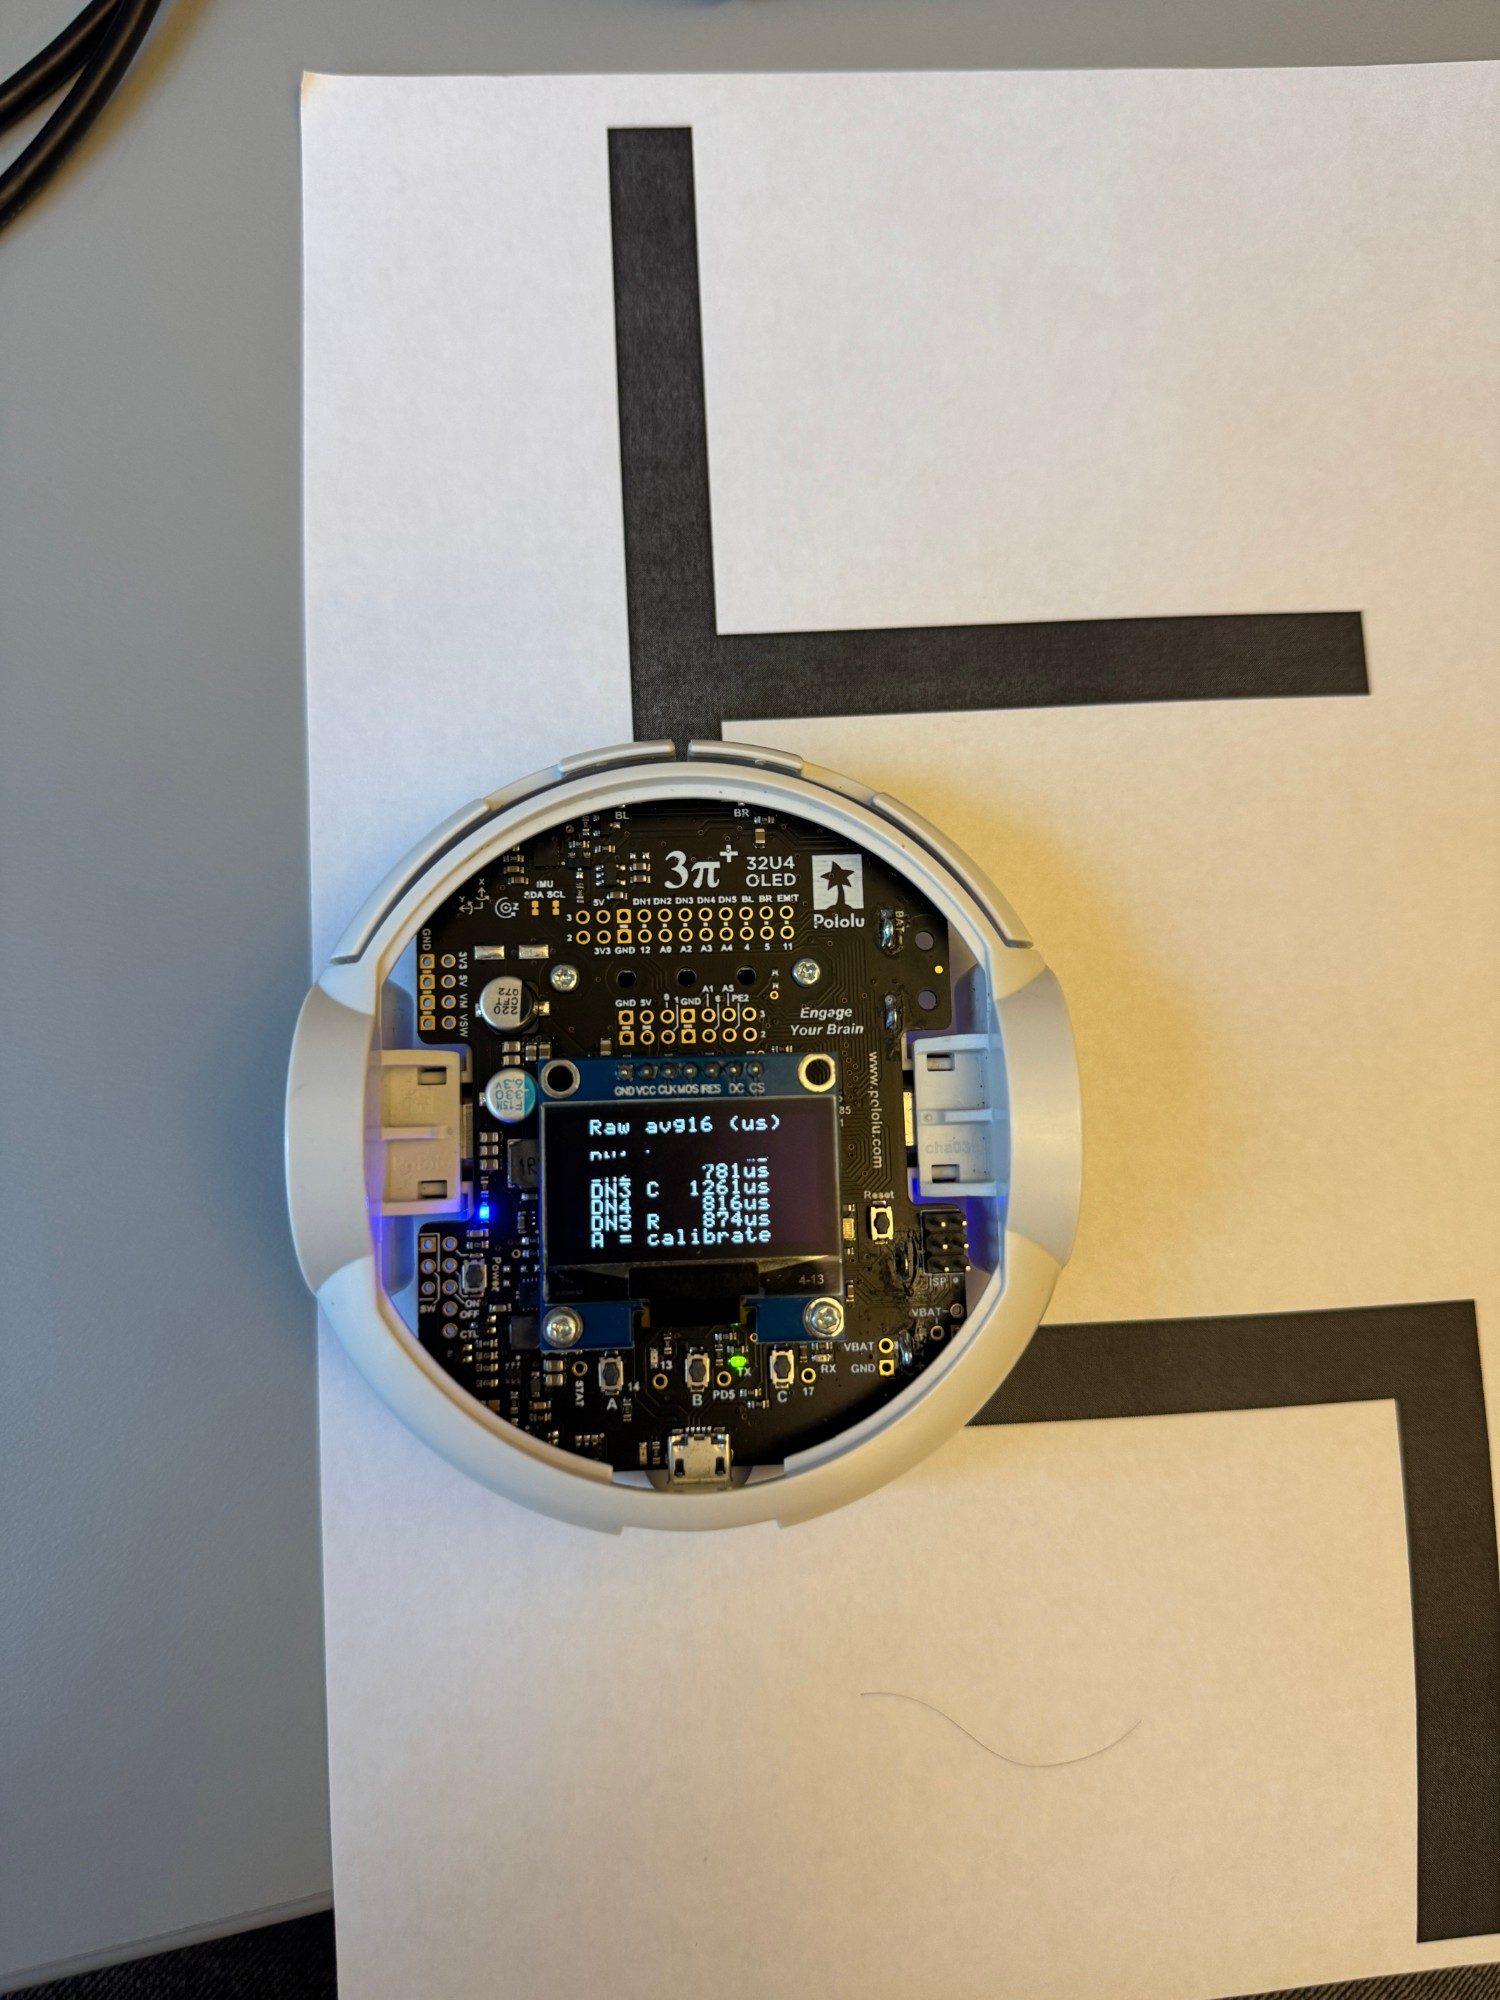
\includegraphics[width=\textwidth]{angle_0deg.jpg}
    \caption{Straight}
  \end{subfigure}\hfill
  \begin{subfigure}{0.40\textwidth}
    \centering
    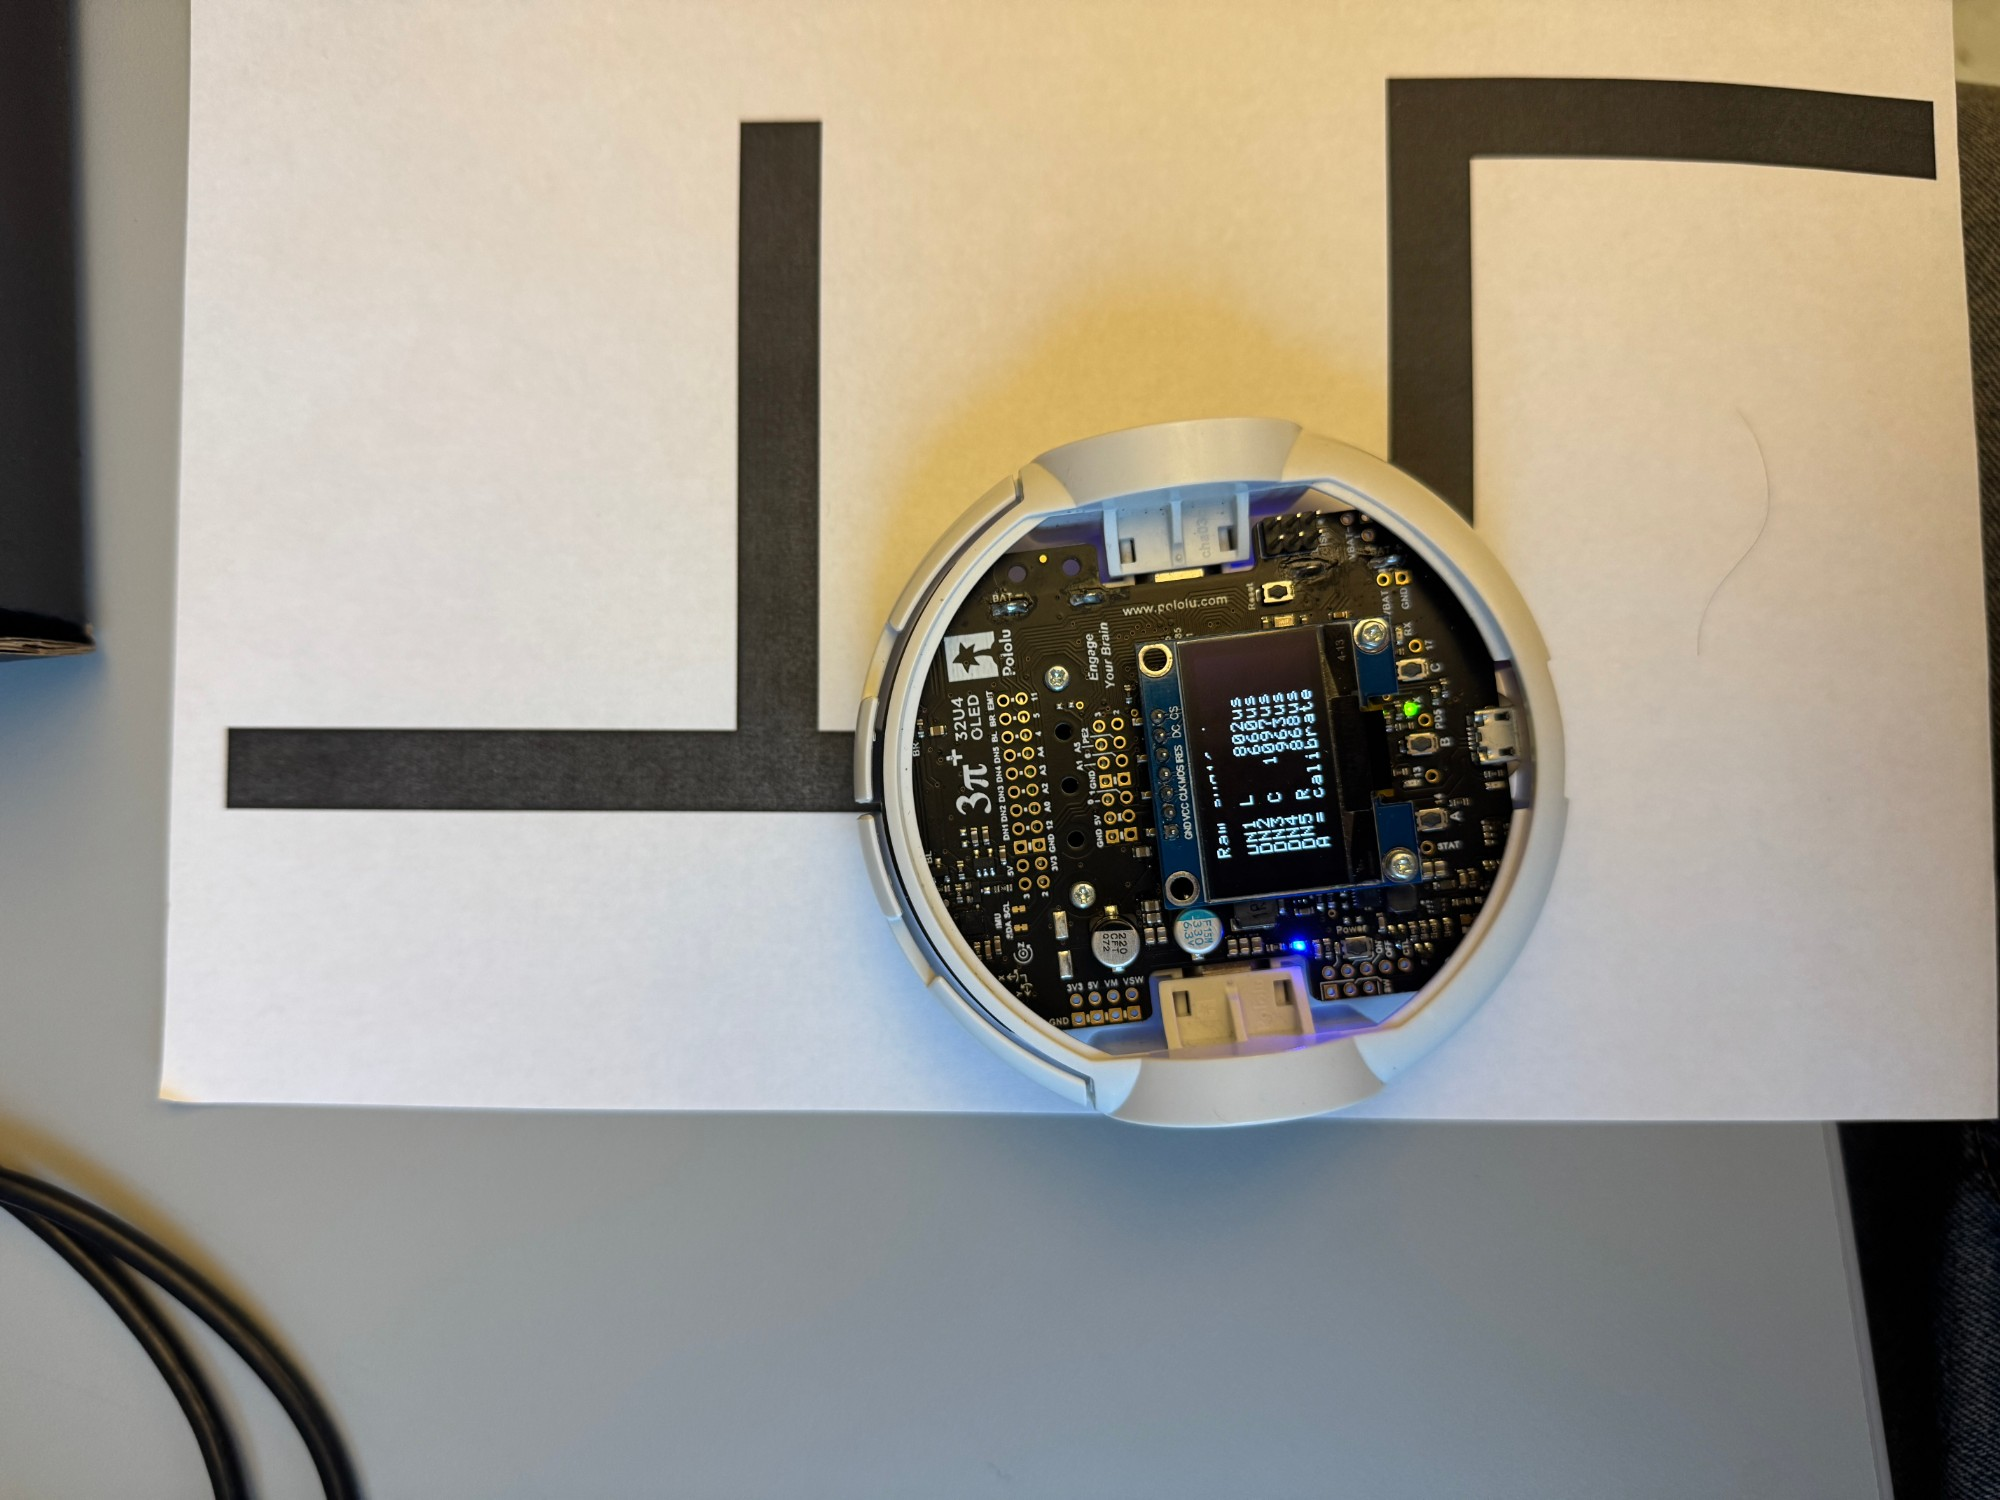
\includegraphics[width=\textwidth]{angle_5deg.jpg}
    \caption{5\textdegree{} (photo rotated)}
  \end{subfigure}\hfill
  \begin{subfigure}{0.26\textwidth}
    \centering
    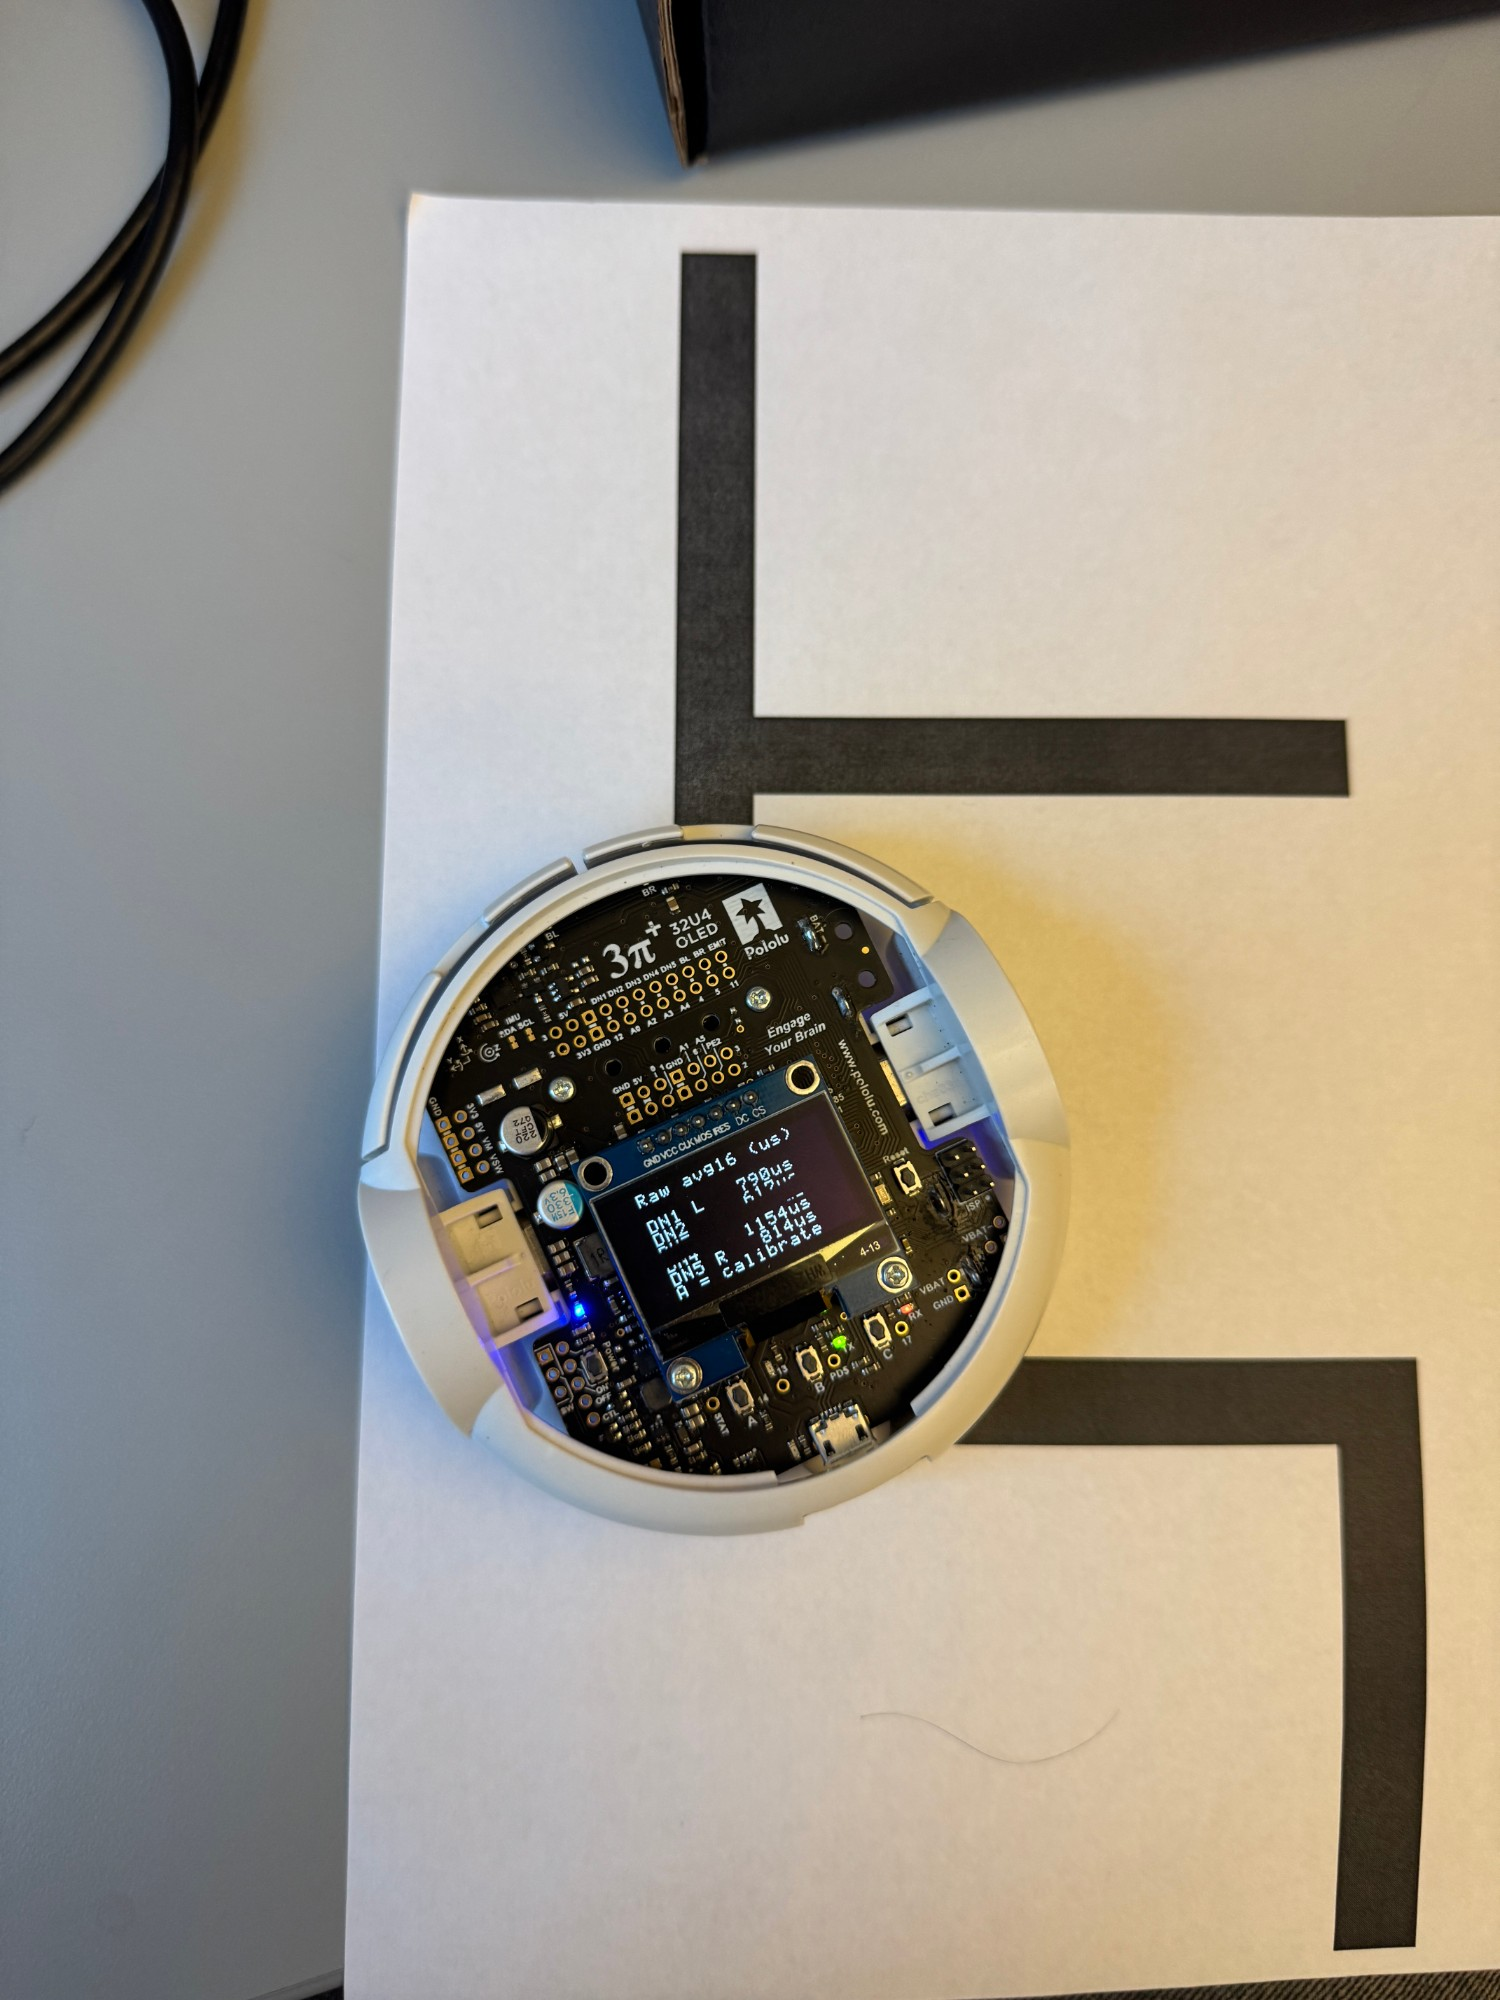
\includegraphics[width=\textwidth]{angle_15deg.jpg}
    \caption{15\textdegree}
  \end{subfigure}
  \caption{Robot placements for the angle experiment.}
  \label{fig:angles}
\end{figure}

\end{itemize}

\section{Results}
\subsection{Bright and Dark Surfaces}

\begin{table}[H]
  \centering
  \caption{Discharge times on white paper, each an average of 16 readings ($\mu$s).}
  \label{tab:white}
  \begin{tabular}{lrrrrrr}
    \toprule
    Sensor & Trial 1 & Trial 2 & Trial 3 & Trial 4 & Trial 5 & Average \\
    \midrule
    DN1 (left)   & 780 & 772 & 782 & 782 & 797 & 783 \\
    DN2          & 600 & 601 & 593 & 596 & 606 & 599 \\
    DN3 (center) & 533 & 532 & 530 & 538 & 526 & 532 \\
    DN4          & 702 & 702 & 705 & 765 & 691 & 713 \\
    DN5 (right)  & 858 & 854 & 853 & 870 & 864 & 860 \\
    \bottomrule
  \end{tabular}
\end{table}

\begin{table}[H]
  \centering
  \caption{Discharge times on the black surface ($\mu$s). Dashes are readings that could not be read from the photos.}
  \label{tab:black}
  \begin{tabular}{lrrrrrr}
    \toprule
    Sensor & Trial 1 & Trial 2 & Trial 3 & Trial 4 & Trial 5 & Average \\
    \midrule
    DN1 (left)   & 2048 & 2065 & --   & 1959 & 2041 & 2028 \\
    DN2          & 2150 & 2146 & 2165 & 2114 & 2112 & 2137 \\
    DN3 (center) & 2038 & 1910 & 1947 & 1976 & 1957 & 1966 \\
    DN4          & 2540 & 2502 & 2661 & --   & 2555 & 2565 \\
    DN5 (right)  & 2196 & 2207 & 2252 & --   & 2260 & 2229 \\
    \bottomrule
  \end{tabular}
\end{table}

\begin{table}[H]
  \centering
  \caption{Contrast between the white and black averages.}
  \label{tab:contrast}
  \begin{tabular}{lrrrr}
    \toprule
    Sensor & White ($\mu$s) & Black ($\mu$s) & Black $-$ white & Black / white \\
    \midrule
    DN1 (left)   & 783 & 2028 & 1246 & 2.59 \\
    DN2          & 599 & 2137 & 1538 & 3.57 \\
    DN3 (center) & 532 & 1966 & 1434 & 3.70 \\
    DN4          & 713 & 2565 & 1852 & 3.60 \\
    DN5 (right)  & 860 & 2229 & 1369 & 2.59 \\
    \bottomrule
  \end{tabular}
\end{table}

\subsection{Angle to a Line}
Each reading $t_i$ was converted to a darkness from 0 (white) to 1 (black) using that sensor's averages from Table~\ref{tab:contrast}, and the line's position $x$ across the sensors was taken as the darkness-weighted average of the sensor positions $p_i$:
\begin{equation}
  d_i = \frac{t_i - W_i}{B_i - W_i}, \qquad
  x = \frac{\sum_i d_i \, p_i}{\sum_i d_i}, \qquad
  p_i = -30, -10, 0, +10, +30~\text{mm}.
  \label{eq:position}
\end{equation}
The sensor positions come from Pololu's control board drawing: DN2--DN4 are 10~mm apart, and DN1 and DN5 are 30~mm from the center and sit about 12~mm behind the other three. Positive $x$ means the line is to the right of center.

\begin{table}[H]
  \centering
  \caption{Readings with the robot on the line ($\mu$s), darkness $d_i$, and line position $x$.}
  \label{tab:angle}
  \begin{tabular}{lrrrrrr}
    \toprule
    Placement & DN1 & DN2 & DN3 & DN4 & DN5 & $x$ (mm) \\
    \midrule
    Straight   & --  & 781  & 1261 & 816  & 874  & $-0.5$ \\
    \quad $d_i$ & --  & 0.12 & 0.51 & 0.06 & 0.01 & \\
    5\textdegree{} & 802 & 660 & 1097 & 963 & 868 & $+1.1$ \\
    \quad $d_i$ & 0.02 & 0.04 & 0.39 & 0.14 & 0.01 & \\
    5\textdegree{}, other way & -- & -- & 1015 & 798 & 876 & -- \\
    15\textdegree{}, both ways & \multicolumn{5}{c}{not readable} & -- \\
    \bottomrule
  \end{tabular}
\end{table}

The values were read from photos of the OLED. Several photos were taken while the screen was being redrawn, so some rows were cut off or shifted against their labels. Those values are marked with dashes. Both 15\textdegree{} readings were affected, so no numbers could be taken from them.

\section{Post-Lab}
\question{Comment on any unexpected behaviors exhibited by the sensors during the experiments.}
\begin{itemize}
\item \textbf{DN4 reads high.} DN4 was about 34\% slower than DN3 on white and 30\% slower on black. A second robot running the same code did not show this, so the difference is in this robot's hardware, not the program. Its black/white ratio (3.60) matches DN2 (3.57) and DN3 (3.70), so DN4 is not weak; every reading is scaled up by about the same factor. This is normal part-to-part variation in the phototransistor or capacitor, and it cancels out when each sensor is normalized with its own white and black averages (Equation~\ref{eq:position}).
\item \textbf{The outer sensors have less contrast.} DN1 and DN5 have a black/white ratio of 2.59, against 3.57--3.70 for the inner three. Both outer sensors read slower on white, which points to their position: they sit about 12~mm behind the inner row, near the edge of the shell.
\item \textbf{Black was nowhere near the timeout.} The black surface read about 2.0--2.6~ms, far below the 10~ms timeout, so black was only 2.6--3.7 times slower than white. The black box lining still reflects a fair amount of IR.
\item \textbf{A sensor centered on the line reads only halfway to black.} With the robot straight, DN3 read 1261~$\mu$s ($d = 0.51$), even though the line was directly under it. Each sensor sees a spot wider than the 1~cm line, so it averages the line and the paper around it. DN2 also read slightly dark ($d = 0.12$).
\end{itemize}

\question{Describe and comment on the results of part 3 above.}
\textbf{Experiment 1:} every sensor's readings were repeatable within about $\pm$2\% on white, except one 765~$\mu$s reading on DN4 (9\% above its other trials). White averaged 532--860~$\mu$s and black 1966--2565~$\mu$s. Every sensor separates white from black clearly, but each needs its own white and black values before the sensors can be compared.

\textbf{Experiment 2:} going from straight to 5\textdegree{} moved the line from $x = -0.5$~mm to $x = +1.1$~mm: DN3 dropped from 1261 to 1097~$\mu$s and DN4 rose from 816 to 963~$\mu$s. The second 5\textdegree{} placement, turned the other way, also lowered DN3 (1015~$\mu$s) while DN4 stayed near white (798~$\mu$s), and DN2 showed a four-digit value that was cut off in the photo, so the line most likely moved toward DN2. The darkened neighbor therefore shows which way the robot is turned.

One reading cannot show the angle directly. The line crosses the sensor row over a width of $1~\text{cm} / \cos\theta$, which is 10.0, 10.04 and 10.35~mm at 0\textdegree, 5\textdegree{} and 15\textdegree, a difference far smaller than the 10~mm sensor spacing. What the readings do show is how far the line moved sideways: when the robot turns by $\theta$ about a point a distance $L$ behind the sensors, the sensors swing sideways by $L \sin\theta$. The 5\textdegree{} trial moved $x$ by 1.6~mm, about 0.3~mm per degree. That is less than expected for the sensors' distance from the robot's center, probably because each sensor's wide view averages the line over a large area (which flattens the weighted average) and because the robot was not turned exactly about its center. With the 15\textdegree{} readings lost, this scale could not be checked at a second angle. Taking a second reading after moving the robot a known distance $D$ along the line, $\theta = \arctan(\Delta x / D)$, avoids both problems and gives the sign of the angle.

\section{Discussion/Conclusion}
All five 3pi+ reflectance sensors were read in parallel by charging their capacitors, releasing them together, and timing each discharge with Timer3. White surfaces read 532--860~$\mu$s and black 1966--2565~$\mu$s, with DN4 consistently slow and the outer sensors less sensitive, so each sensor needs its own white and black calibration. A single reading shows where the line is under the robot and which way the robot is turned, but the angle itself is better measured from the change in line position between two readings.

\pagebreak

\appendix
\section{Full Code}
\label{app:code}

% Read straight from the Lab8 project so the listings always match the code.
% \footnotesize so long comment lines fit.
\lstinputlisting[basicstyle=\ttfamily\footnotesize,caption={Raw, calibration and line screens (main.c).},label={app:main}]{../../Lab8/main.c}

\lstinputlisting[basicstyle=\ttfamily\footnotesize,caption={Sensor interface and pin map (sensors.h).},label={app:sensorsh}]{../../Lab8/sensors.h}

\lstinputlisting[basicstyle=\ttfamily\footnotesize,caption={Parallel sensor reading with Timer3 (sensors.c).},label={app:sensorsc}]{../../Lab8/sensors.c}

\lstinputlisting[basicstyle=\ttfamily\footnotesize,caption={Calibration and line position interface (line.h).},label={app:lineh}]{../../Lab8/line.h}

\lstinputlisting[basicstyle=\ttfamily\footnotesize,caption={Calibration and line position (line.c).},label={app:linec}]{../../Lab8/line.c}

\lstinputlisting[basicstyle=\ttfamily\footnotesize,caption={Button A interface (button.h).},label={app:buttonh}]{../../Lab8/button.h}

\lstinputlisting[basicstyle=\ttfamily\footnotesize,caption={Button A input with debouncing (button.c).},label={app:buttonc}]{../../Lab8/button.c}

\lstinputlisting[basicstyle=\ttfamily\footnotesize,caption={Course-provided OLED driver header, with OLED\_writeTextLine() added (OLED.h).},label={app:oledh}]{../../Lab8/OLED.h}

\lstinputlisting[basicstyle=\ttfamily\footnotesize,caption={Course-provided OLED driver, with OLED\_writeTextLine() added (OLED.c).},label={app:oledc}]{../../Lab8/OLED.c}

\end{document}
